\documentclass[]{IEEEtran}
% some very useful LaTeX packages include:
%\usepackage{cite}      
\usepackage{graphicx}   
\usepackage{subfigure} 
\usepackage{url}       
\usepackage{amsmath}    
\usepackage{caption2}
% Your document starts here!
\begin{document}

% Define document title and author
	\title{Weekly Report}
	\author{Adviser: Prof. Yang Wen \\Student: Cheng Wensheng\\ Period: 2018.4.8-4.15
	}
	\markboth{Visual Information Processing Group}{}
	\maketitle

% Write abstract here
\begin{abstract}
	This week I mainly put my effort on writing IP search report and reviewing the ISPRS Journal paper.
\end{abstract}

% Each section begins with a \section{title} command
\section{Paper Review}
	% \PARstart{}{} creates a tall first letter for this first paragraph
	\PARstart{T}{he} paper combined superpixel segmentation algorithm with multiscale CNN, then proposed the per-superpixel MCNN method for high spatial resolution remote sensing image classification. The author compared this method with traditional OBIA method and per-pixel CNN method in several respects. 
	\begin{itemize}
		\item Per-superpixel MCNN method outperformed others in 	accuracy. 
		\item Per-superpixel MCNN method cost less time than others.
		\item Per-superpixel MCNN method consumed less storage space than other methods. 
	\end{itemize}

	The major concerns are the novelty and the contribution to remote sensing field. As author claimed, the per-superpixel MCNN method was its main contribution. However, as far as I know, there are already plenty of works which combine superpixel with CNN, i.e., using superpixel to segment image, then classifying these image patches with CNN. It’s a very common practice. It’s not qualified as the innovation point of this paper.
	
	Besides, for the multi-scale CNN method, it uses images with different sizes containing the same object to train several CNNs. In nature, it utilizes low level features and high level features. This idea is used widely in CNN, such as FCN and DeepLab. The latter integrate low layer’s output with high layer’s output in one CNN without training multiple CNNs for different scales. Obviously, the multi-scale method of FCN and DeepLab is much leaner than the proposed MCNN.
	
	Fig.~\ref{fig:mp} is the superpixel dataset. Fig.~\ref{fig:ss} is the multi-scale CNN architecture.

\newpage
\begin{figure}[!hbt]
%		 Center the figure.
		\vspace{2cm}
%		\hspace{50cm}
		\begin{center}
			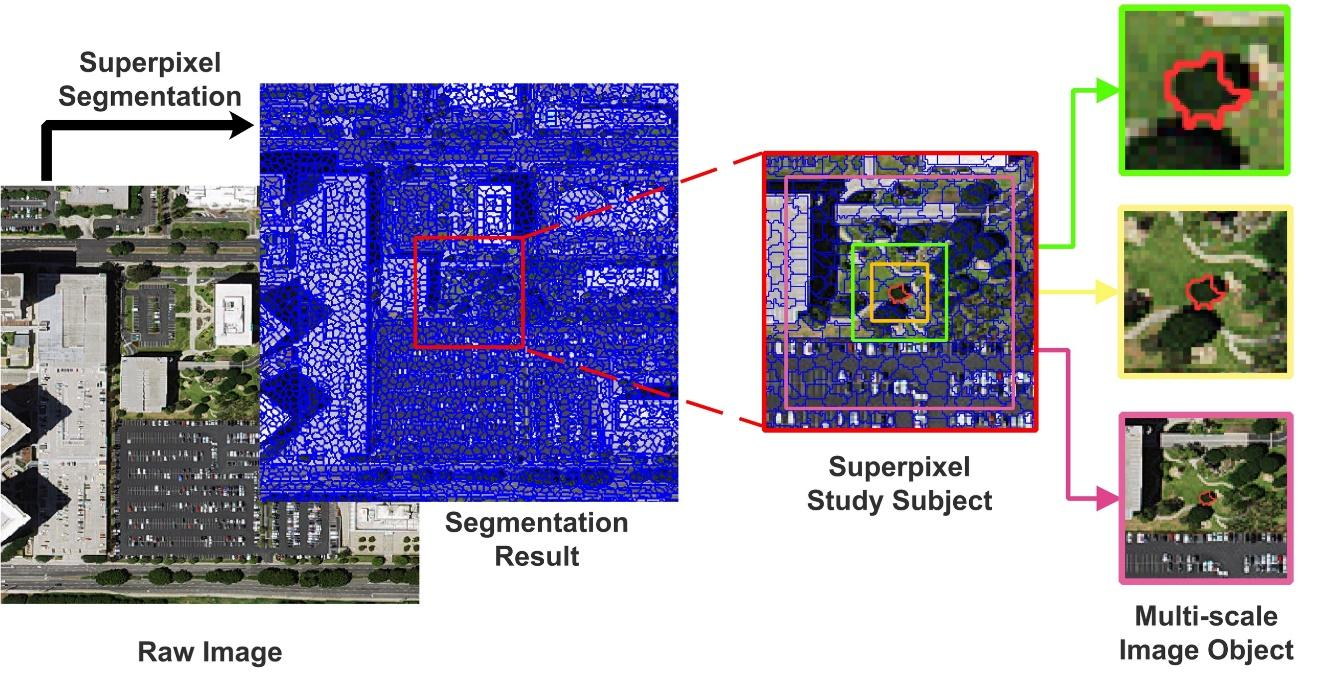
\includegraphics[width=\columnwidth]{superpixel_dataset}
				%		 Create a subtitle for the figure.
			\caption{Superpixel dataset}
			\label{fig:mp}
		    \vspace{1cm}
			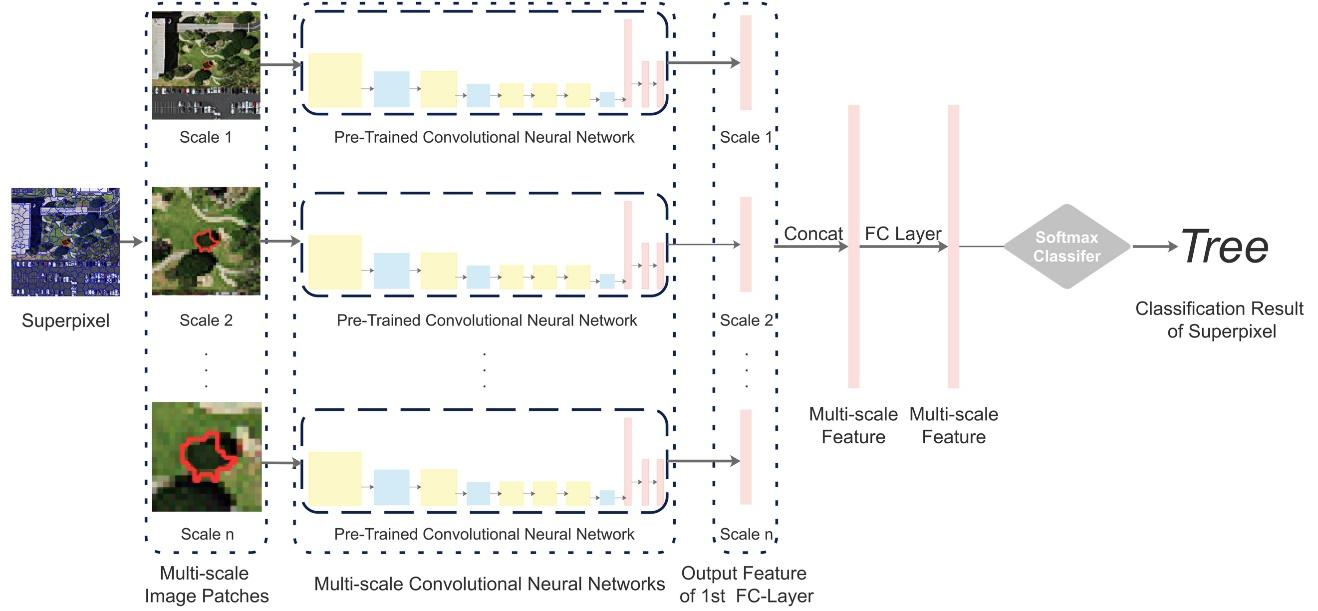
\includegraphics[width=\columnwidth]{multi-scale_CNN}
				%Create a subtitle for the figure.
			\caption{Multi-scale CNN architecture}
			\label{fig:ss}
		\end{center}
	\end{figure}

% Your document ends here!
\end{document}